\section{ReproBLAS}
  \label{sec:reproBLAS}
  ReproBLAS is the name given to our beloved library of implementations of algorithms described in this paper.
  The code is available online at \texttt{<http://bebop.cs.berkeley.edu/reproblas>}.
  To be useful to the greatest number of performance-conscious scientific software developers, ReproBLAS is written in C (conforming to the C99 Standard \cite{c99}, with calling conventions that are compatible with the data types of the C89 Standard \cite{c89}).
\begin{comment}
 complex types \cite{c89} as discussed in \cite{cblasinterface}
Because the C89 standard did not standardize the complex floating point type, all interfaces refer to complex types using \texttt{void*} pointers. If a function would normally return a complex type, a \texttt{void*} pointer is added as the last argument and the function name is suffixed by \texttt{_sub}
\end{comment}
  The choice of C allows for intrepid Fortran and C++ users to take advantage of the library as well.
  Code generation and testing utilities are implemented in the more productive language Python \cite{Python}.
  A few distributed memory functions are supplied using MPI \cite{MPI}, the industry standard for distributed memory programming.

  We leave the specifics of the library to the documentation included with the library itself, and here offer only a summary of some of the design decisions made in ReproBLAS.

  Several of the functions in ReproBLAS are optionally vectorized using Intel AVX or SSE intrinsics \cite{SSEAVX}, depending on what is available on the system. With AVX, vectorization allows for 256-bit registers (4 \texttt{double} or 8 \texttt{float}) to be operated on in one instruction. Because so many routines were vectorized and due to the complicated nature of the operations, a Python suite was implemented to generate code that is generic to the particular vectorization in question. By simply augmenting this suite of code generation functions, this allows for future modifications of ReproBLAS to use newer intrinsics (such as AVX-512) when they become widely available. Another benefit of code generation is that it allows us to programatically restructure code to take advantage of loop unrolling and instruction-level parallelism.

  To handle the complex build processes involved in code generation without increasing the software requirements of the library, we created a custom build system written entirely in GNU Make. We adopted the build system from a non-recursive makefile template called nonrec-make \cite{nonrec-make}. The build system handles some of the complexity of code generation with the help of the Python package Cog \cite{Cog}, which allows the programmer to write Python code inline with C code.

  Code generation and cache blocking add several parameters to ReproBLAS that must be tuned. OpenTuner \cite{OpenTuner}, an extensible Python autotuner, was used to search the parameter space to find optimal values for ReproBLAS parameters.

  ReproBLAS is divided into several modules, each one with a separate header file and static library. \texttt{idxd.h} contains the primitive operations discussed in Section \ref{sec:primitiveops} and the utility functions regarding the indexed type discussed in Section \ref{sec:indexed}. 
\texttt{idxd.h} also contains several basic functions not mentioned that relate to the core reproducible summation algorithm.
 \texttt{idxdBLAS.h} contains the indexed versions of the BLAS functions discussed in Section \ref{sec:compositeops}.
 These functions are optimized composite operations built from functions in \texttt{idxd.h}.
 \texttt{reproBLAS.h} contains versions of functions in \texttt{idxdBLAS.h} that do not require the user to use indexed types.
 Each function has the same name and signature as its BLAS counterpart, and behaves similarly (except with added guarantees of reproducibility).
 Functions in \texttt{reproBLAS.h} with an ``r'' prepended to their name allow the user to specify the number of accumulators ($K$, where the internal indexed type used is $K$-fold) used to compute the result, allowing for a user-specified level of accuracy. 
\texttt{idxdMPI.h} contains MPI data types used to communicate indexed types, and also contains an MPI reduction operator allowing the user to reproducibly reduce the MPI indexed types.
  \subsection{Timing}
  All timings are performed on a blah machine with a hot cache. we compare against MKL BLAS. ALl matricies are represented in column-major order
  \subsubsection{Difficult Input}
    Because the reproducible summation algorithm needs to perform additional operations (Algorithm \ref{alg:update}) if the maximum absolute value of the data increases during summation, the runtime depends (up to a constant factor) upon the input. To show the differences in runtime, we show the time it takes to reproducibly sum $2^20$ \texttt{double} and \texttt{float} from two different datasets. The first data set is an easy case, the uniform distribution from 0 to 1. The second data set is the most difficult possible case, numbers (alternating in sign to avoid infinities) increasing in absolute value exponentially starting at the minimum positive floating point value and ending with the largest positive finite floating point value. This data set is difficult because the exponent of the maximum absolute value increases linearly from its minimum to its maximum possible value. Therefore, the Update operation (Algorithm \ref{alg:update}) must be performed more frequently to adjust the index of the indexed type. We can compare this to the uniform distribution in $[0, 1)$, which very quickly achieves a number (greater than $0.5$) that has the largest floating point exponent possible from the distribution. After such a number is seen, no more updates need to be performed. The timings are displayed in Figure \ref{fig:easy_vs_hard_timings}
  \begin{figure}[H]
  \begin{center}
  \includegraphics[width=\textwidth]{plots/easy_vs_hard.pdf}
  \caption{Time taken to sum $2^{16}$ floating point numbers of varying difficulty.}
  \label{fig:easy_vs_hard_timings}
  \end{center}
  \end{figure}
  \subsubsection{BLAS1}

    We show how our reproducible summation stacks up against a simple $C$ \texttt{for}-loop in Figure \ref{fig:forloop_timings}. Time (measured relative to the peak theoretical time for recursive summation) is shown for each method. The numbers to be summed are normally distributed with mean $0$ and variance $1$. For several good reasons (lack of vectorization, lack of loop unrolling, etc.) the \texttt{for}-loop is not running at peak. With this in mind, reproducible summation is competetive with a simple \texttt{for}-loop.
  \begin{figure}[H]
  \begin{center}
  \includegraphics[width=\textwidth]{plots/sum_comparison.pdf}
  \caption{Relative floating point summation time}
  \label{fig:forloop_timings}
  \end{center}
  \end{figure}
    To give a comparison to a BLAS1 function, we show in Figure \ref{fig:dot_timings} timings of the reproducible dot product versus the Intel Math Kernel Library \cite{MKL} BLAS dot product. Again, the data is distributed such that the products of the two input vectors are normally distributed with mean $0$ and variance $1$.
  \begin{figure}[H]
  \begin{center}
  \includegraphics[width=\textwidth]{plots/dot_comparison.pdf}
  \caption{Relative dot product time}
  \label{fig:dot_timings}
  \end{center}
  \end{figure}
  \subsubsection{BLAS2}
    We show in Figure \ref{fig:gemv_timings} timings of the reproducible matrix-vector product versus the Intel Math Kernel Library \cite{MKL} BLAS matrix-vector product. The data is distributed such that the products of elements of the input vector and elements of the matrix are normally distributed with mean $0$ and variance $1$.
  \begin{figure}[H]
  \begin{center}
  \includegraphics[width=\textwidth]{plots/gemv_comparison.pdf}
  \caption{Relative matrix-vector product time}
  \label{fig:gemv_timings}
  \end{center}
  \end{figure}
  The non-transposed matrix-vector product is the only case where composition of BLAS2 and BLAS3 functions did not achieve close to optimal results. Because the reproducible dot product operates most efficiently on contiguous sections of memory, the matrix must be transposed so that memory can be read contiguously. This causes the reproducible matrix-vector product to perform poorly due to the extra cost of matrix transposition in an already memory-bound routine. In future versions of the library, this method could be improved by writing a custom inner-loop.

  The transposed matrix-vector product performs better than the non-transposed case. Timings are shown in Figure \ref{fig:gemv_trans_timings}. The reader should notice that in this case, the reproducible routine is only about a factor of two times slower than the optimized BLAS routine.
  \begin{figure}[H]
  \begin{center}
  \includegraphics[width=\textwidth]{plots/gemv_comparison.pdf}
  \caption{Relative matrix-vector product time}
  \label{fig:gemv_timings}
  \end{center}
  \end{figure}

  \subsubsection{BLAS3}
    We show in Figure \ref{fig:gemm_timings} timings of the reproducible matrix-matrix product versus the Intel Math Kernel Library \cite{MKL} BLAS matrix-matrix product. The data is distributed such that the products of elements of one input vector and the other are normally distributed with mean $0$ and variance $1$. Because the timings for each transposition case (transposing or not transposing $A$ or $B$) are similar, we show only the standard case for brevity. In this case, since both routines are running close to peak, the reproducible routine is about a factor of 8 times slower than the optimized BLAS routine.
  \begin{figure}[H]
  \begin{center}
  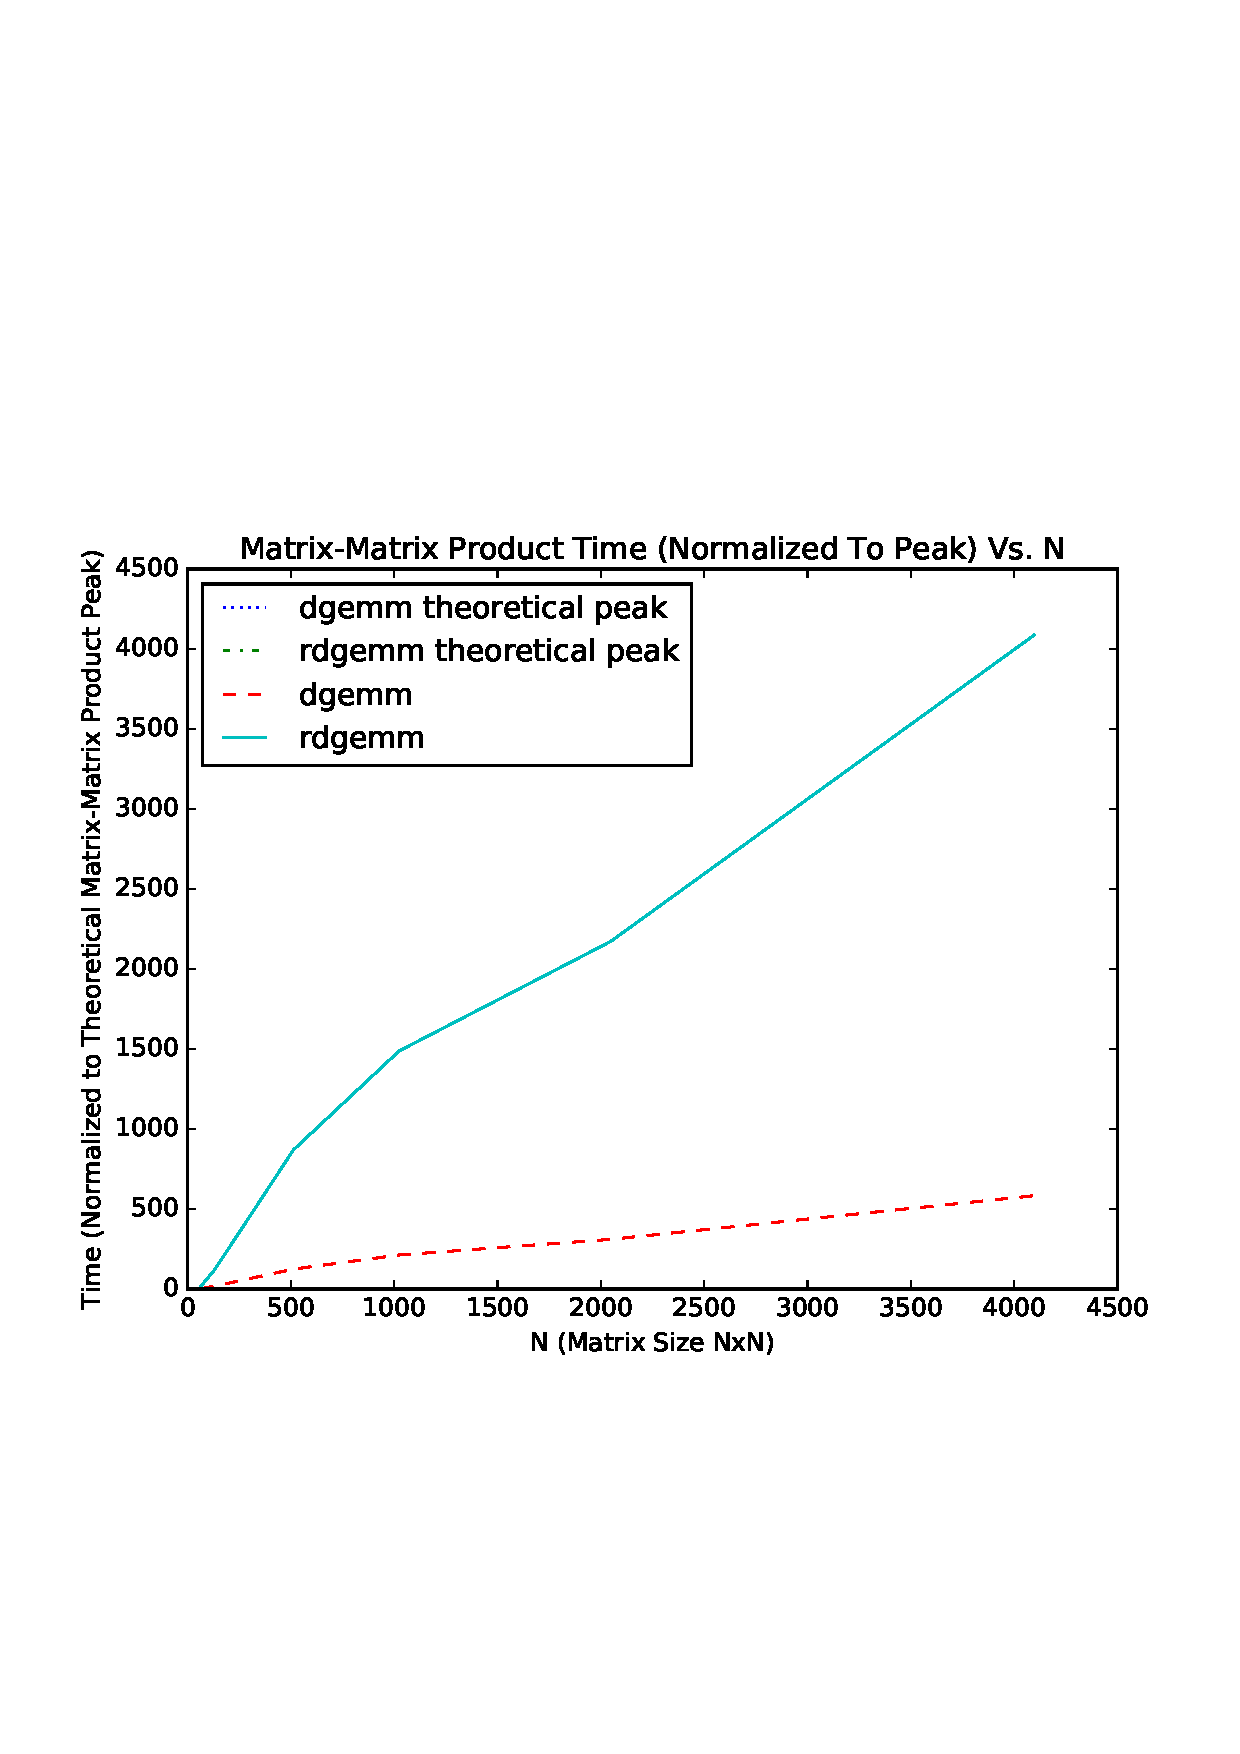
\includegraphics[width=\textwidth]{plots/gemm_comparison.pdf}
  \caption{Relative matrix-matrix product time}
  \label{fig:gemm_timings}
  \end{center}
  \end{figure}

  \subsection{Testing}
  In understanding the testing methodology behind ReproBLAS, is important to distinguish between the matrics of reproducibility and accuracy. Although high accuracy can sometimes result in reproducibility, it is not a guarantee. For this reason, we test the accuracy and the reproducibility of the ReproBLAS methods separately.

  Testing in ReproBLAS starts with the BLAS1 methods (\textt{sum}, \textt{asum}, \textt{nrm2}, \textt{dot}). These methods are first checked to see that their results are accurate, then checked to see if the results are reproducible.

  The accuracy of the reproducible BLAS1 methods is validated by checking to see if the results of each method are within the error margin specified by \eqref{} from the true results. Because the true summation result must be known, these tests are performed on distributions with known sums. The input vectors used are shown in Table \ref{}. 
  \begin{enumerate}
    \item A full period of a sine wave (this sums to zero).
    \item 
  \end{enumerate}
  Because the reproducible summation methods operate on bins, we repeat the accuracy tests on scaled versions of the input data set $W$ times, each time increasing the scale by a factor of two. This allows us to test many different cases where sums are split across bin boundaries. This is performed on data very close to overflow to test cases where the data is split between bin 0 and bin 1. This is also performed on data very close to underfow to test cases where some data is lost due to underflow.

  To validate the accuracy of the methods in the presence of \texttt{Inf}, \texttt{-Inf}, and \texttt{NaN}, the reproducible BLAS1 methods are tested on the vectors shown in Table \ref{}.

  After validating the accuracy of the reproducible BLAS1 methods, their reproducibility is verified. Each method is checked to see if it produces the same result under several different permutations of data.The data is permuted by reversing, sorting (in ascending or descending order of value or absolute value), or random shuffling. To check that the result is independent of blocking, the data is grouped into several blocks and each block is operated on separately, then the results for each block are combined using the appropriate function. Several different block sizes are tested for each permutation of the data.

  Once the BLAS1 methods are tested, the results of BLAS2 and BLAS3 (\texttt{gemv} and \texttt{gemm}) methods are tested against reference versions. These reference versions use no blocking and are simple to understand and code.

  Several parameters must be tested in the BLAS, including the increment between elements of a vector, row or column major ordering of matricies, whether or not to transpose matricies, and scaling factors on vectors and matricies. Because there are several parameters that need testing, a Python test harness was created to easily test each combination of values for these parameters.

